\documentclass[a4paper,12pt,fleqn]{article}%fleqn pour aligner les equations à gauche
\usepackage{../../Styles/Cours}

\newcommand{\chnum}{Chapitre 7}
\newcommand{\chtitle}{De l'analogique au numérique}
\newcommand{\dtype}{Activité}

\begin{document}
\maketitle
Pour enregistrer et stocker du son sur un summort numérique, toute une chaîne d'acquisition est nécessaire. Elle aboutit à un signal numérique.

\begin{figure}[h!]
    \caption{La chaîne de transmission et de stockage du son}
	\centering
	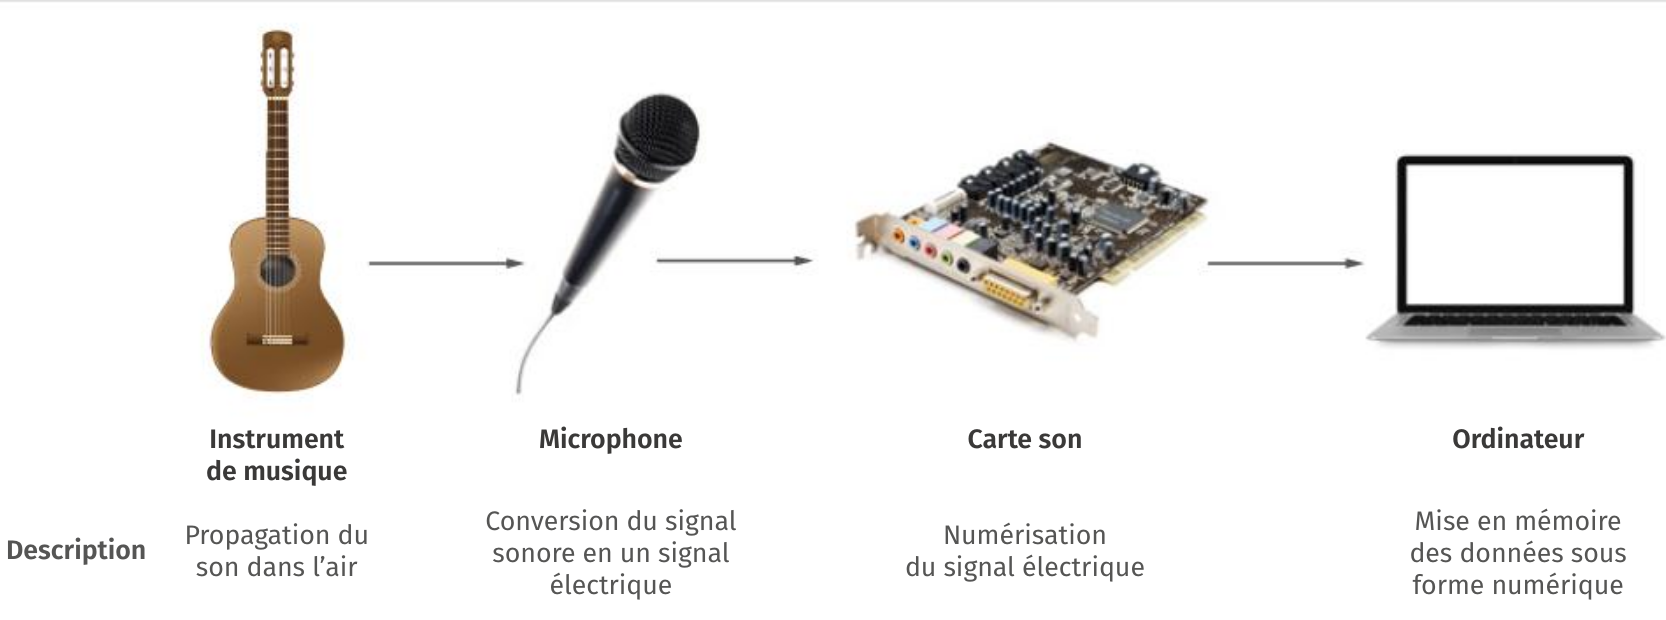
\includegraphics[width=.8\linewidth]{Ressources/1ES_C7_Act1_Fig1.png}
\end{figure}

\begin{figure}[h!]
    \caption{Numérisation d'un son : Échantillonnage}
    \centering
    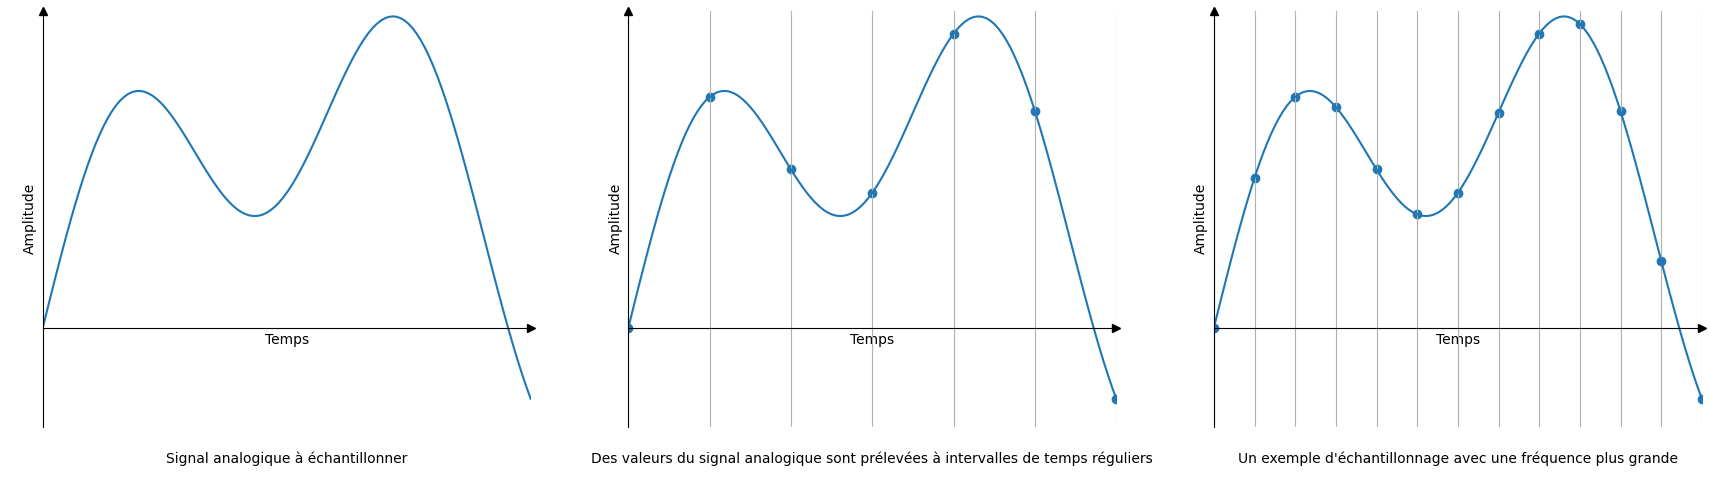
\includegraphics[width=.8\linewidth]{Ressources/1ES_C7_Act1_Fig2.png}
\end{figure}

\begin{figure}[h!]
    \caption{Numérisation d'un son : Quantification}
    \centering
    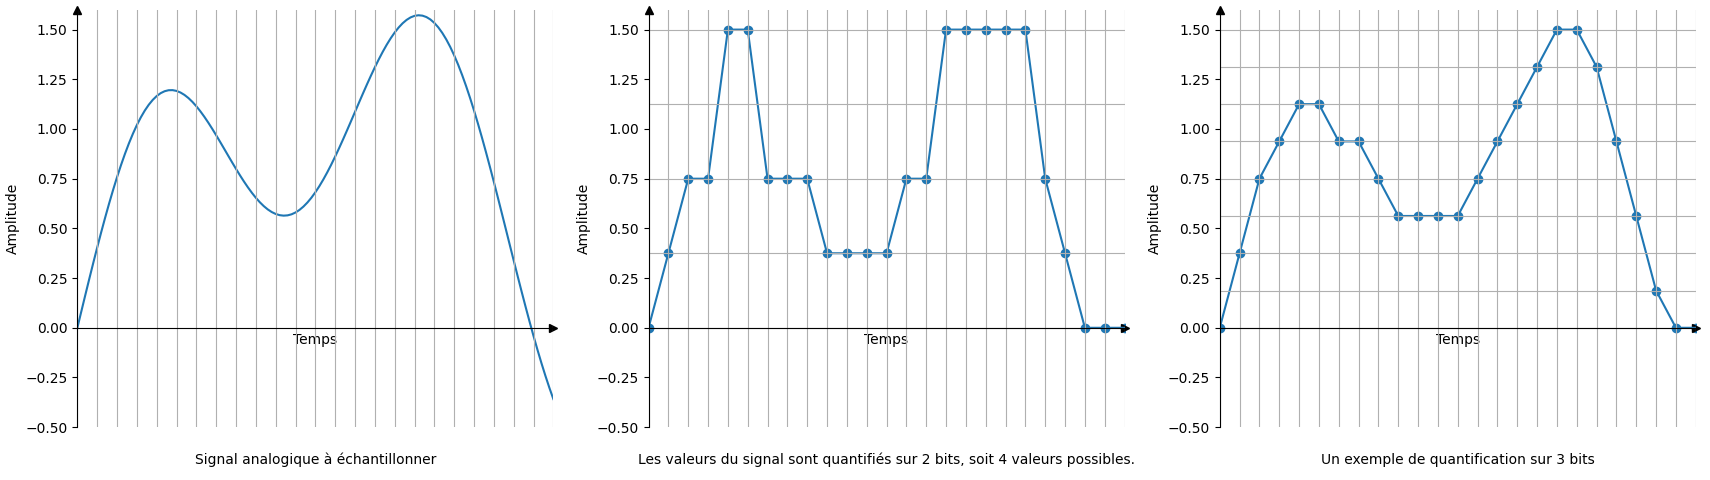
\includegraphics[width=.8\linewidth]{Ressources/1ES_C7_Act1_Fig3.png}
\end{figure}

\begin{figure}[h!]
    \caption{La qualité d'acquisition}
    \begin{minipage}{.58\linewidth}
        Lorsque l'on enregistre une musique à l'aide d'un logiciel (comme Audacity), la fréquence d'échantillonnage par défaut est de \SI{44,1}{kHz} et la quantification des échantillons est réalisée sur \SI{16}{\bit}. Si l'on enregistre en mode stéréo, deux voies sont alors créées (un canal droit et un canal gauche).\\
        Il existe différents formats permettant d'améliorer la qualité d'enregistrement des sons et de se rapprocher au mieux du son entendu en studio. L'audio haute résolution (HRA) est un format d'enregistrement avec un encodage sur \SI{24}{\bit} et un échantillonnage pouvant aller jusqu'à \SI{192}{kHz}.
    \end{minipage}
    \begin{minipage}{.38\linewidth}
    	\centering
    	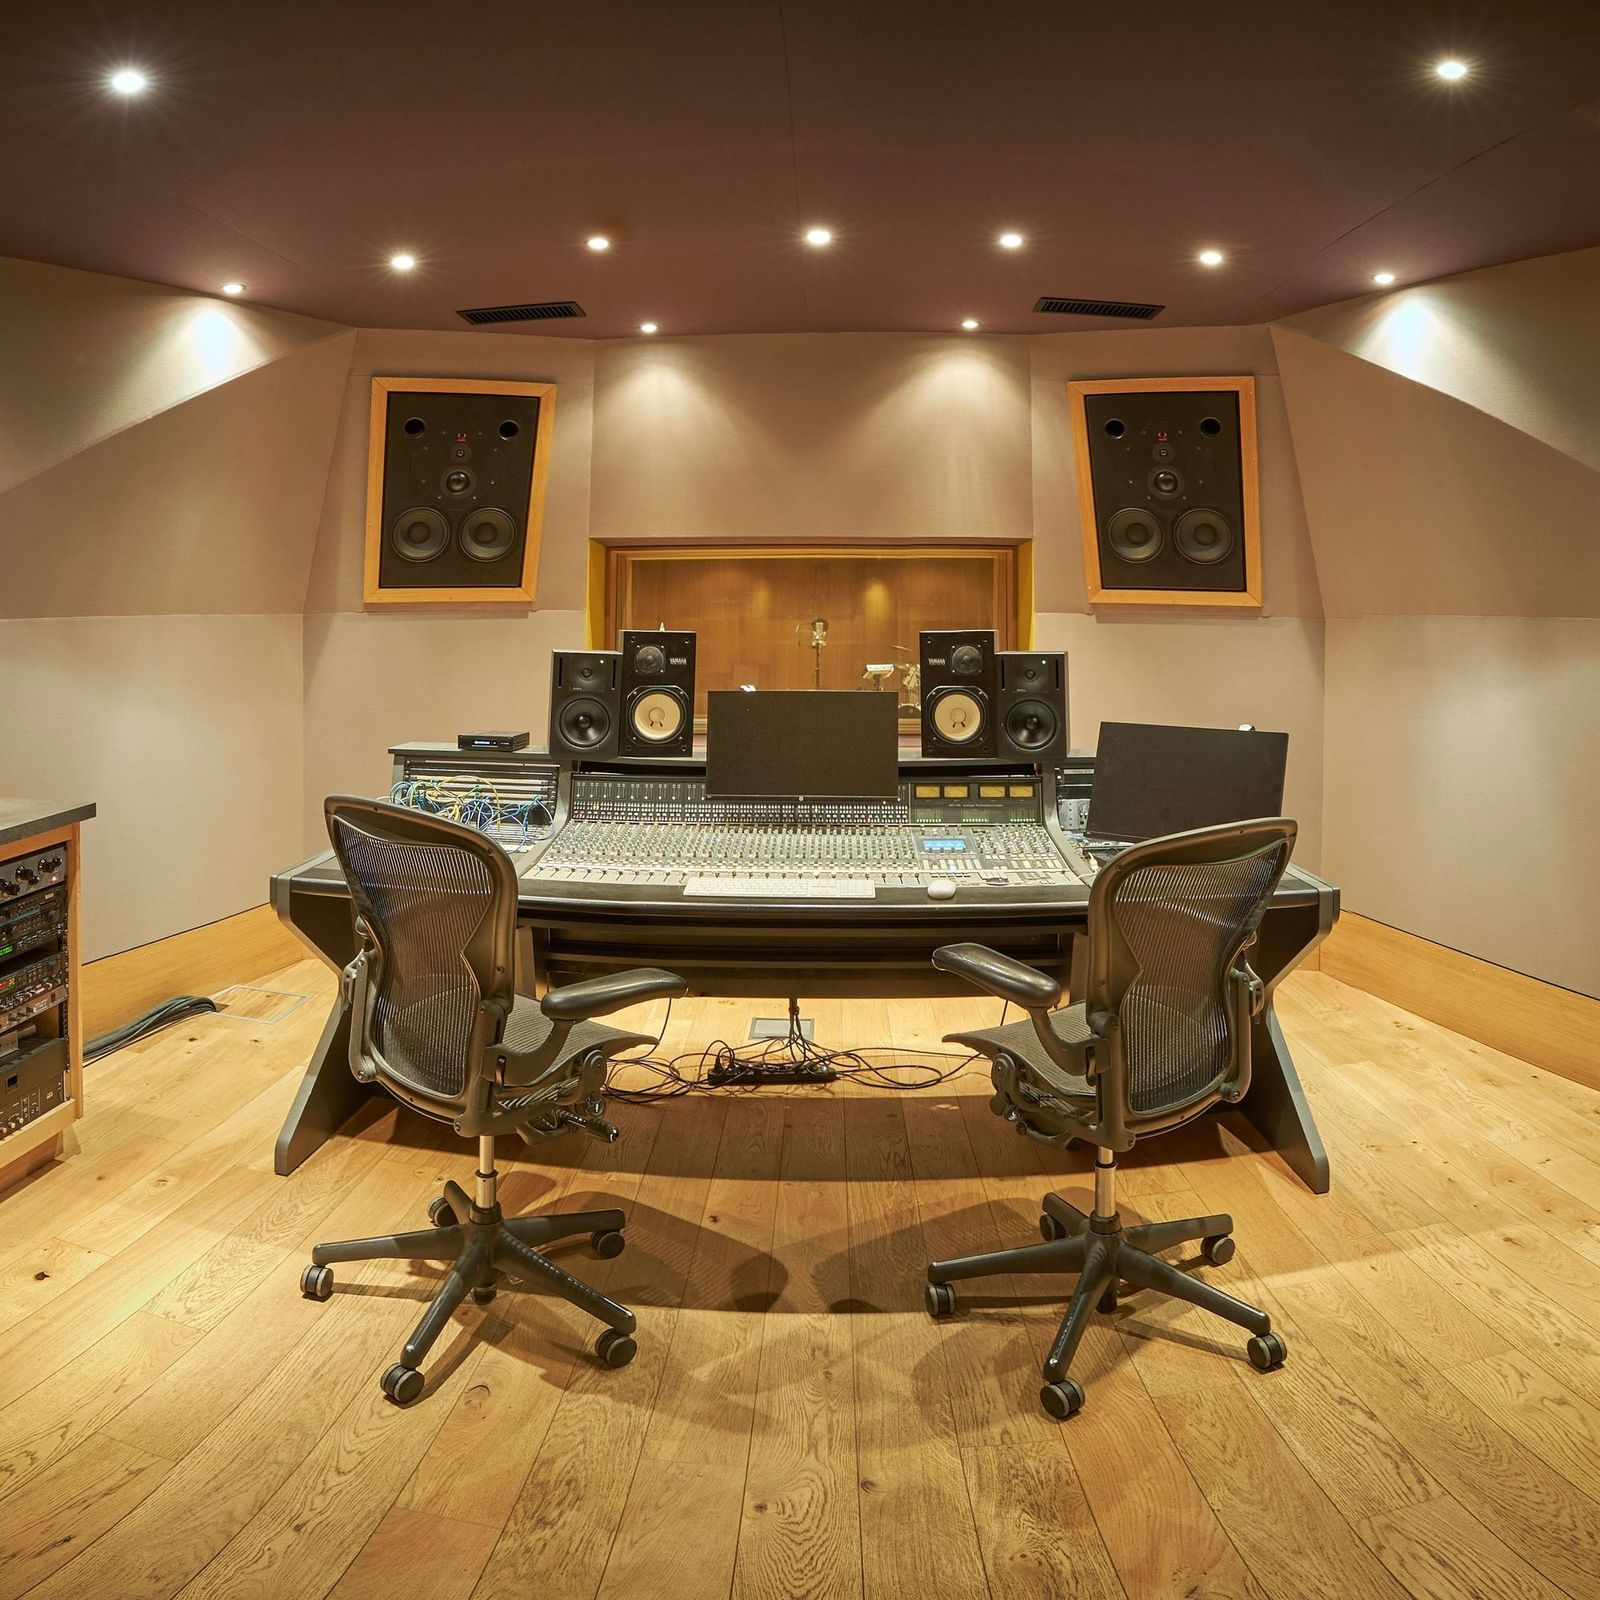
\includegraphics[width=.8\linewidth]{Ressources/1ES_C7_Act1_Fig4.jpg}
    \end{minipage}
\end{figure}

\begin{figure}[h!]
	\caption{Les caractéristiques du CD audio}
	\centering
	\begin{tabular}{|c|c|c|}
		\hline
		\textbf{Capacité de stockage} & \textbf{Fréquence d'échantillonnage} & \textbf{ Quantification}\\
		\hline
		\SI{700}{Mo} & \SI{44,1}{\kilo\hertz} & \SI{16}{\bit}\\
		\hline
	\end{tabular}
\end{figure}

\textbf{Questions :}
\begin{enumerate}
	\item Identifier le ou les élément(s) de la chaîne d'information pour lesquels le signal est cous forme analogique. Faites de même pour ceux où le signal est sous forme numérique.
	\item Comparer les trois graphiques. Préciser l'impact de la fréquence d'échantillonnage $f_e$ sur le signal numérique.
	\item Comparer les trois graphiques. Déduisez-en l'impact de la quantification sur la ressemblance entre le signal numérique et le signal analogique.
	\item listez les conditions nécessaires pour qu'un signal numérisé soit le plus fidèle possible au signal analogique.
	\item La formule suivante permet de calculer la taille d'un fichier audio d'une certaine durée. Traduire celle-ci par une phrase.
\end{enumerate}
\begin{center}
	\begin{tabular}{c|l}
		\multirow{5}{*}{$t=f_e \cdot n \cdot \Delta t \cdot N_{voies}$} & $t$ : taille du fichier (\unit{\bit})\\
		& $f_e$ : fréquence d'échantillonnage (\unit{\hertz})\\
		& $n$ : nombre de bits pour  la quantification (\unit{\bit})\\
		& $\Delta t$ : durée de l'audio (\unit{\second})\\
		& $N_{voies}$ : nombre de voies (mono ou stéréo)\\
	\end{tabular}
\end{center}
\begin{enumerate}[resume]
	\item Calculer la taille d'un fichier audio d'une durée d'une seconde dans le cas d'un son numérique sur un CD.
	\item À partir de la question précédente, déduire la durée maximale de musique stockable sur un CD.
	\item Finalement, faites le lien entre la fidélité du son numériqé et la taille du fichier. Argumenter votre réponse.
\end{enumerate}

\end{document}